\chapter{Future Works}
\label{sec:future}
\section{Role-Based Access Control (RBAC)}
In the present version of our project, we did not include the Role-Based Access Control. In Role-Based Access Control (RBAC), rights and permissions are assigned to roles rather than to individual users. 

A general scenerio for RBAC model has been presented in Figure 5.1.
\begin{figure}[h]
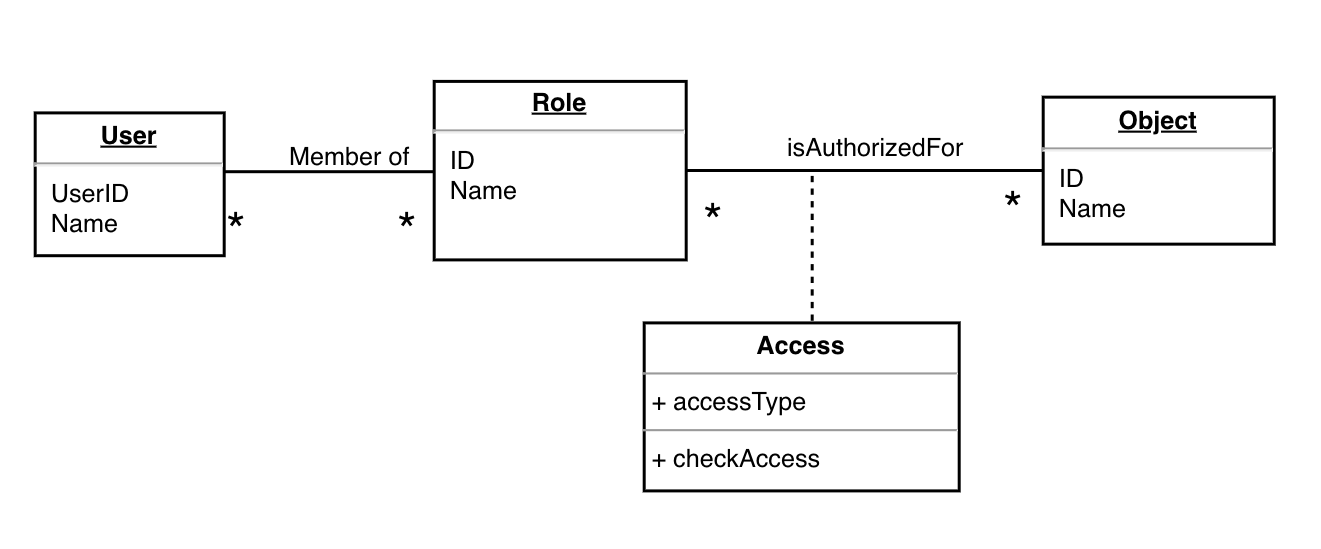
\includegraphics[width=14cm]{content/A.png}
\centering
\caption{General scenerio when using RBAC}
\end{figure}


RBAC can be added to SoftProj model using these following steps:

\subsection*{Step 1:}
The first thing to do is to identify the operations and objects which should be controlled using RBAC. The resources which we need to control access in our system is:
\begin{itemize}
\itemsep-1.3em 
    \item View artifacts
\item Rate Artifacts
\item Review Artifacts
\item Access Review Template
\end{itemize}




\subsection*{Step 2:}
Roles have to be identified because the permissions of access will be according to Roles not Users. In our system, there could be 5 roles. 
\begin{itemize}
\itemsep-1.3em 
    \item Lecturer
    \item RPM
    \item Reviewer
    \item Submitter
    \item Admin
\end{itemize}




\subsection*{Step 3:}

The next step is assigning people to a different role. This is an important step because People can have a different role but at a time one may not have more than a single role. We will apply Static Separation of Duty (SSD) and Dynamic Separation of Duty (DSD)  both. 

\begin{itemize}
\itemsep-1em 
    \item \textbf{SSD}
    \begin{enumerate}
     \itemsep-1em 
    \item The Lecturer, RPM, and Admin cannot be a submitter. If they want to be a submitter then they will not have access as other roles.
    \item RPM himself/herself cannot be Reviewer.
    
\end{enumerate}

    \item \textbf{DSD}
    \begin{enumerate}
    
    
\itemsep-1em 
    \item A submitter/team can be a Reviewer but they can not review their own artifacts.
    \item A Lecturer can be an RPM sometimes but he/she will not be allowed to rate himself/herself.
    
\end{enumerate}
\end{itemize}


The roles may change over time. It would be more beneficial if we change the roles as required, or add new ones when really necessary. 


\newpage

\subsection*{Step 4:}
Finally, we need to make an access system according to the roles:
\begin{enumerate}
    
    
\itemsep-1em 
    \item  A submitter will have access only to the artifacts created by his/her team.
\item  A lecturer will have access to all artifacts. The lecturer should be able to see the status of all artifacts under review, and the results of reviews for all previously reviewed artifacts. 
\item  A Review Project Manager (RPM) will have access only to the artifacts of the teams assigned to the RPM by the lecturer. 
\item  A reviewer will have access only to the artifact that is assigned to him/her.
\item  Admin will have access to all the artifacts.

    
\end{enumerate}